\documentclass[10pt,conference]{IEEEtran}

% Font
\usepackage{lmodern}
%\usepackage[T1]{fontenc}

\usepackage{bbm}
\usepackage{bm} % Bold math
\usepackage{mathtools}
\usepackage{listings}
\usepackage{amsmath}
\usepackage{amssymb}

\usepackage{hyperref}
\usepackage{graphicx}	% For figure environment
\usepackage{makecell}	% For multiline cells in tables
% \usepackage{subfig}
\usepackage{subcaption}

% For the figures
\usepackage{pgfplots}
\pgfplotsset{compat=1.17}
\usepackage{changepage}
\usepackage{tikz}
\usepackage{pgf}
\usetikzlibrary{graphs, shapes}

% justify text in bibliography
\usepackage{ragged2e}  % for \justifying
\usepackage{etoolbox}
\apptocmd{\thebibliography}{\justifying}{}{}
% links in blue
\definecolor{links}{HTML}{2A1B81}
\hypersetup{colorlinks=true,citecolor=blue,linkcolor=,urlcolor=links}

\renewcommand\P[1]{\mathbb{P}\!\left\{#1\right\}}
\newcommand\given{\:\middle|\:}

\newcommand\tl[1]{\{\text{Label} = #1\}}
\newcommand\pl[1]{\{\text{Pred} = #1\}}
\newcommand\tp{\{\text{Pred} = 1 \cap \text{Label} = 1\}}
\newcommand\fp{\{\text{Pred} = 1 \cap \text{Label} = 0\}}
\newcommand\tn{\{\text{Pred} = 0 \cap \text{Label} = 0\}}
\newcommand\fn{\{\text{Pred} = 0 \cap \text{Label} = 1\}}


\begin{document}
\title{{\LARGE Automatic detection of available area for rooftop solar panel installations}\vspace{-3mm}}    

\author{
  Alexander \textsc{Apostolov} (\texttt{alexander.apostolov@epfl.ch})\\
  Auguste \textsc{Baum} (\texttt{auguste.baum@epfl.ch})\\
  Ghali \textsc{Chraibi} (\texttt{ghali.chraibi@epfl.ch})\\
  \\
  Supervisor: Roberto \textsc{Castello} (\texttt{roberto.castello@epfl.ch})\\ EPFL Laboratory of Solar Energy and Building Physics\\
  \\
  \textit{CS-433 Machine Learning --- December 2020, EPFL, Switzerland}
}
\maketitle

\begin{abstract}
%TODO explain why it is important an that we are the first ones to do it
%Say we also labelled
  In this report we propose and analyze a neural network for automatic detection of available rooftop solar panel installations on aerial images. We focus on tuning the network and on analyzing methods to use its outcome to make decisions.
  %TODO state results of best model
\end{abstract}

\section{Introduction}
%TODO change name
\subsection{Importance of the task}

\subsection{Data}
The dataset used consists of ortho-rectified [**TODO should explain ?**] images of Geneva canton, Switzerland provided by the Swiss Federal Office of Topography. The images are split in tiles corresponding to different region of the canton. Images are $250 \times 250$ pixels, RGB arrays saved in png format. Each pixel correspond to $0.25 \times 0.25 \text{ m}^2$.


\section{Models and Methods}

\subsection{Data labelling}
%Updated tool labelled images ourselves, show strange example
We labelled X images using an updated version of an existing labelling tool based on OpenCV~\cite{Castello_2019}. The tool of this paper is used to label solar panels which are usually rectangular, we update it for our task by making it easy to select regions of an image (usually a roof) and then extruding parts of it (parts of the roof not suitable for solar panels). Each pixel that belongs to a rooftop where there is available space to place solar photovoltaic panels are classified as \emph{PV pixels}, whereas the other pixels are classified as \emph{no-PV pixels}, they do not correspond to rooftop or there are obstacles that do not allow to place any photovoltaic panels on it (e.g. chimney, pipe, windows, etc.).

The labelled images were chosen from a randomized subset of the dataset mentioned above, taken from different tiles (area) of the canton in order to have the most representative variety of rooftop shapes and types (industrial, old town, center town, countryside, etc.). 

\subsection{Data preprocessing}

\subsubsection{PV images vs. no-PV images}
In this paper, we distinguish PV images that contain at least some PV pixels from no-PV images that contain only no-PV pixels. We separate images in different folders as we want to manipulate precisely with how much no-PV images we train our model. We suppose it can have an impact for the robustness of our model, reinforcing the rejection of false positives.  

\subsubsection{Data augmentation}
As we don’t have a lot of samples, we apply a random transformation on each sample (image and label) to artificially enlarge our dataset. The transformation is composed of :  
\begin{itemize}
	\item a random square crop which takes at least 60\% of the sample and is then resized to the size of the original sample
	\item a horizontal flip of the sample which happens with probability 0.5
\end{itemize}
  
\subsubsection{Training, validation, test split}
We split the dataset into a train, validation and test set in the following proportion 70\%/15\%/15\%.

The transformation mentioned above is only applied to the training set as we want to test our models on the original distribution. For the same reason, we use the original ratio of PV images / no-PV images for the validation set and the test set and alter this ration only when training the model.

\subsection{U-Net}
Computer vision tasks are commonly tackled using convolutional networks. 
Here we propose to use a special convolutional network called a \textbf{U-Net},~\cite{ronneberger2015unet}
introduced in 2015 for image segmentation in biomedical imaging.
We choose to use this model as it can yield state-of-the-art results with only few images.
The U-Net as shown in \autoref{fig:UNetarchitecture} consists of two parts,
the contracting and the expanding path.
% Pas sur de comprendre cette phrase
The former is used to \textit{detect features} on an image
and the latter to \textit{find the locality} of these features in the original space.

The contracting path we use consists of 5 stages where we apply two $3 \times 3$ convolutions padded by 1 pixel on each side,
each followed by a batch normalization layer and a rectified linear unit.
We use the same number of channels as described in \autoref{fig:UNetarchitecture}, namely 64, 128, 256, 512 and 1024 for each stage of the contracting path. 
Stages in the contracting path are separated by a $2 \times 2$ max-pooling layer with a stride of 2. 

The expanding path we use consists of 4 stages starting by an upsampling by a factor of 2 and a $2 \times 2$ convolution to halve the number of channels,
a copy of the feature map in the corresponding stage of the contracting path is concatenated and then $3 \times 3$ convolutions padded by 1 pixel on each side are applied,
each followed by a batch normalization layer and a rectified linear unit.
We use the same number of channels per stage as in \autoref{fig:UNetarchitecture}, namely 512, 256, 128 and 64.

The model terminates by a $1 \times 1$ convolution to a feature map with only one channel.
From this output we can compute, for each pixel, the probability that it represents an area that is available for a solar panel.

\begin{figure}[tbp]
    \centering
    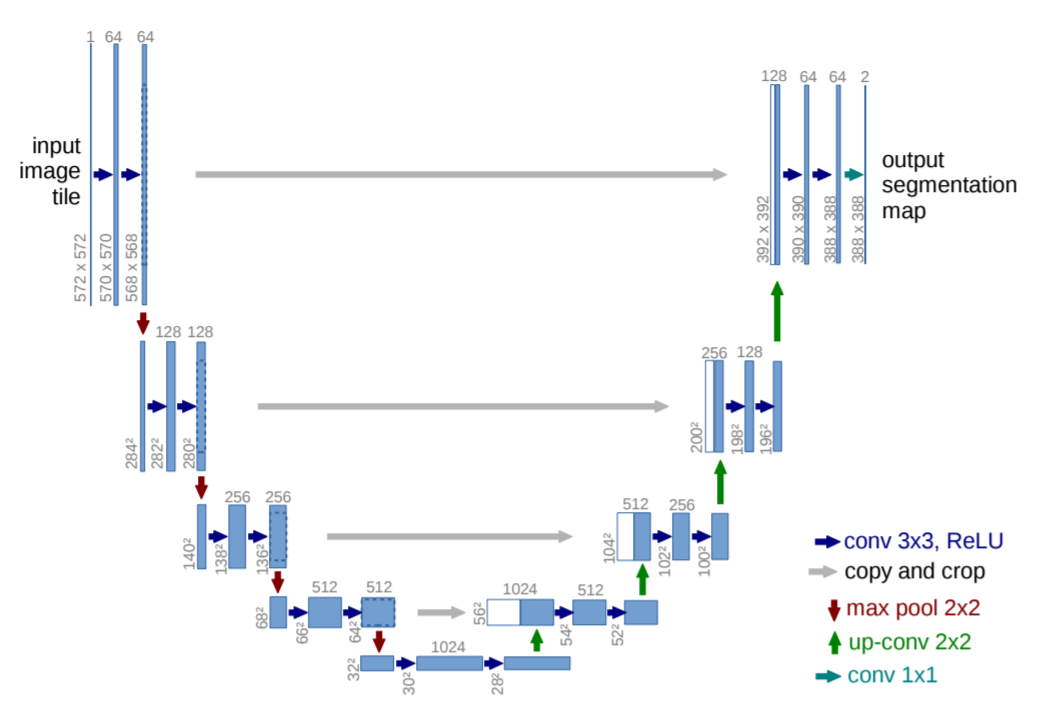
\includegraphics[width=\columnwidth]{report/images/UNet.png}
    \caption{
        U-Net example as described in the original paper~\cite{ronneberger2015unet}.
        Each blue box corresponds to a multi-channel feature map; the number of channels is found on top of the box, and the dimensions are at the lower left edge of the box.
        White boxes represent copied feature maps.
        The arrows denote the different operations.
    }
    \label{fig:UNetarchitecture}
\end{figure}

\subsection{Loss}\label{loss}
Our model has to classify each pixel into 2 classes, either the area is available for a rooftop solar panel or not. We try the following three losses:
\begin{itemize}
    \item Binary cross entropy (BCE)
    \item Weighted binary cross entropy (wBCE)
    \item L1 loss
\end{itemize}
Because the U-Net outputs an arbitrary value in $\mathbb{R}$ for each pixel, we apply a sigmoid layer before computing the loss.

The weighted binary cross entropy can be used when there is a significant class imbalance, which is indeed the case here:
most pixels are not available for rooftop solar panels. 
The formula for this loss is:
\begin{equation*}
    %L = \frac{1}{N} \sum_{n=1}^N l_n, \\
    L = \frac{1}{N} \sum_{n=1}^N  [py_n \log(\sigma(x_n))
        + (1-y_n) \log(1-\sigma(x_n))],
    %l_n = - [py_n \log(\sigma(x_n))
        %+ (1-y_n) \log(1-\sigma(x_n))]
\end{equation*}
where $x_n$ and $y_n$ are respectively the output of the model and the true class (0 or 1) for pixel $n$,
and $p$ is the weight given to the positive class. 
Setting $p>1$ increases the recall, whereas $p<1$ increases the precision.
As described in the documentation of PyTorch we set this weight as
% $\frac{\text{\#negative pixels}}{\text{\#positive pixels}}$
$\frac{\mathrm{support}(0)}{\mathrm{support}(1)}$
in the dataset.


\subsection{Training}
We train the model with different parameters and choose the best combination which has the best results on the validation set. We vary the following parameters:

\subsubsection{Optimizer}
We decide to try Adam~\cite{kingma2014adam} and Stochastic Gradient Descent (SGD) to train the U-Net.

\subsubsection{Effect of using noPV images during training}
We try using different amounts of noPV images during training. We think that using too little might make for a model which doesn't generalize well, while using too much might bias the model. We measure the amount of noPV images by considering the percentage of noPV images compared to PV images in the train set. The percentageswe consider are $0\%, 25\% \text{ and } 50\%$.

\subsubsection{Loss}
We use the three losses mentioned in \autoref{loss}. For the weighted cross entropy loss we use a different weight based on the percentage of noPV images we use in the train set. We compute the following weight using the formula from \autoref{loss}.
\begin{center}
    \begin{tabular}{||c | c||} 
        \hline
        Percentage noPV & Weight for wBCE\\ [0.5ex] 
        \hline\hline
        $0\%$ & $5.13$ \\
        \hline
        $25\%$ & $6.46$ \\
        \hline
        $50\%$ & $8.10$ \\
       % [1ex] 
        \hline
    \end{tabular}
\end{center}

\subsubsection{Learning rate scheduling}
We try different constant values of the learning rate of the optimizer. However, small values tend to reach a better minimum of the loss function but very slowly, while big values are faster but don't guarantee a good convergence. We propose to use a learning rate scheduler to combine the best of both. We start training with a larger learning rate and decrease it during training.

\subsection{Tuning threshold on probability after training model} \label{ssec:threshold}
Since the model outputs weights (real numbers in all of $\mathbb{R}$),
we use a sigmoid to transform the weights into numbers in $[0,1]$.
Once this is done, we still need to find the best decision boundary---the threshold probability $\theta$ over which a pixel is decided to be available for PV.
For that we perform a grid-search over thresholds, computing the $F_1$-score over our validation set 
for each threshold.
Finally, we compute the median $Q_2(\theta)$ for each threshold and find the one that maximizes this.
%Then, we compute order statistics (first, second and third quartiles) and find the threshold that maximizes the following metric:
%\begin{equation} \label{eq:threshold_metric}
%    f(\theta) = Q_2(\theta) - (Q_3(\theta) - Q_1(\theta))
%\end{equation}
%where $Q_i$ is the $i$\textsuperscript{th} quartile.
%Our reasoning is that while the median $F_1$-score
%should be high, we should also prioritize
%values for which we are more certain of the ``true'' $F_1$-score.


As a reminder, the precision of the prediction
corresponds to $\P{\text{Pred}=1 \given \text{Label} = 1}$ while
the recall corresponds to $\P{\text{Label}=1 \given \text{Pred} = 1}$.
As such, both are susceptible to become undefined if
$\#\tl1 = 0$ or $\#\pl1 = 0$, respectively.

Since we must have noPV images in the validation and test sets in order to faithfully represent real-world usage,
these possibilities must be accounted for.
By default, the precision and recall functions we use
can catch these errors and arbitrarily set the value to
0 or to 1.

Setting the value to 0 in case of noPV is not sensible,
because in this case, even if the model perfectly predicts
all pixels as 0, both precision and recall will be set to 0
(hence so will the $F_1$-score).
However, setting the value to 1 also seems suboptimal, because
then we can't make the difference between a model that
perfectly predicted where a PV area was, and a model
that did any prediction on a noPV image.
In both cases, the $F_1$-score is being influenced artificially.

Another solution was then to compute precision and recall
as weighted averages, as is done with multi-class
problems.
In this case, we compute the metrics 
with 1 as the positive class and also with 0 as the
positive class, and then take a weighted average of
the two; the weights are the support of each class.
That way, division-by-zero issues naturally disappear.
Unfortunately, this tended to give a disproportionate
boost to the precision whereas the recall is not as
affected (in fact, it becomes equal to the accuracy).

Finally, we decided that would be concatenating all the images
in the set and to compute each metric just once.
That way, though we lose out on the statistical power
that computing for each image might bring, we are
certain that no undefined behaviour will occur.

%Despite the issues it had, we went with the we decided the issues it has, w

\subsection{Testing}
Once the best threshold is found, we use this to produce
the final model; we apply this on our test set and compute
standard classification metrics for each prediction,
using the last method presented in \autoref{ssec:threshold}.


Finally, we decided that a good estimator for the
performance would be to concatenate all the images
in t
% is computed as
% \begin{equation*}
%     \text{precision} = \frac{\#\tp}{\#\tl1}
% \end{equation*}
% and the recall as
% \begin{equation*}
%     \text{recall} = \frac{\#\tp}{\#\pl1},
% \end{equation*}
% where $\tl{i}$ corresponds to the set of pixels classified as $i$ is the ground-truth label and 
% $\pl{i}$ corresponds to the set of pixels classified as 1 is the predicted label.

% The $F_1$-score is computed as 
% \begin{equation*}
%     F_1 = 2 \times \frac{\text{precision} \times \text{recall}}{
% \text{precision} + \text{recall}}
% \end{equation*}
% 
% Additionally, we compute the accuracy as
% \begin{align*}
%     \text{accuracy} = \\
%     \frac{\#\tp + \#\tn}{\#\{\text{All}\}}
% \end{align*}
% and the Jaccard loss or intersection-over-union (IoU) as
% \begin{equation*}
%     \text{IoU} = \frac{\#\tp}{\#\{\text{Pred} = 1 \cup \text{Label} = 1\}}.
% \end{equation*}

The way we treat images that are noPV is quite important for
measuring the performance of a model.
Indeed, a number of our models have been trained with few or no
noPV images, whereas the validation and test sets are a more
faithful representation of the data that would be passed to a
production-grade model.

We use the $F_1$-score to find the ``best'' threshold possible, which implies computing the precision and recall.
However, precision is not defined when there are no positive true labels,
and recall is not defined when there are no positive predicted labels.
We could arbitrarily decide to set them to 0 or to 1;
originally it was 0, but it transpired that even if
the model could determine that the image was a noPV, it
would still receive a rating of 0, which seemed unfair.
On the other hand, after changing it to 1, we were
dubious as to whether we could really trust the results
we obtained. Indeed, it would seem easier to predict an
image as noPV than to try and find the PV, but with this
choice the two were rewarded the exact same way; it was
not possible to determine whether the ratings were
good because of the model, or because there were many
noPV images in the test set.

Another solution was to compute precision and recall
as weighted averages, as is done with multi-class
problems. In this case, we compute the metrics 
with 1 as the positive class and also with 0 as the
positive class, and then take a weighted average of
the two; the weights are the support of each class.
That way, division-by-zero issues naturally disappear.
However, this tended to give a disproportionate
boost to the precision whereas the recall is not as
affected (in fact, it becomes equal to the accuracy).

Because the computation of the $F_1$-score is unweighted,
this means that lower threshold values

We computed the metrics for each image in the test set and then computed summary statistics;
however, concatenating all the images and computing each
metric on this one ``super-image'' is also an easy
way to ascertain the performance of our models.
We collected the results using the latter method in
\autoref{tbl:test_results}.
%The size of the validation and test sets is according to the train-validation-test split decided in the
%beginning, namely 15\% of the total dataset for each.

%EXPLAIN HOW THE noPV ARE TREATED (set to 0? set to 1? discarded?)
%Set to 1 

\section{Results}
After selecting appropriate learning rates we choose to train the following models:

\begin{center}
    \begin{tabular}{||c | c  | c | c | c ||} 
        \hline
        $N^o$ & Optimizer & $\%$noPV & Learning rate & Loss \\ [0.5ex] 
        \hline\hline
        1 & ADAM & $0\% $ & $10^{-3}$ & wBCE \\
        \hline
        2 & ADAM & $0\% $ & $10^{-4}$ & wBCE \\
        \hline
        3 & ADAM & $0\% $ & $10^{-3}$ and $10^{-4}$ & wBCE \\
        \hline
        4 & ADAM & $25\% $ & $10^{-3}$  & wBCE \\
        \hline
        5 & ADAM & $25\% $ & $10^{-4}$ & wBCE \\
        \hline
        6 & ADAM & $25\% $ & $10^{-3}$ and $10^{-4}$ & wBCE \\
        \hline
        7 & ADAM & $50\% $ & $10^{-3}$ & wBCE \\
        \hline
        8 & ADAM & $50\% $ & $10^{-4}$ & wBCE \\
        \hline
        9 & ADAM & $50\% $ & $10^{-3}$ and $10^{-4}$ & wBCE \\
        \hline
        10 & SGD & $0\% $ & $10^{-3}$ & wBCE \\
        \hline
        11 & SGD & $0\% $ & $10^{-2}$ & wBCE \\
        \hline
        12 & SGD & $0\% $ & $10^{-2}$ and $10^{-3}$ & wBCE \\
        \hline
        13 & SGD & $25\% $ & $10^{-3}$ & wBCE \\
        \hline
        14 & SGD & $25\% $ & $10^{-2}$ & wBCE \\
        \hline
        15 & SGD & $25\% $ & $10^{-2}$ then $10^{-3}$ & wBCE \\
        \hline
        16 & SGD & $50\% $ & $10^{-3}$ & wBCE \\
        \hline
        17 & SGD & $50\% $ & $10^{-2}$ & wBCE \\
        \hline
        18 & SGD & $50\% $ & $10^{-2}$ and $10^{-3}$ & wBCE \\
        \hline
        19 & ADAM & $0\% $ & $10^{-3}$ and $10^{-4}$ & BCE \\
        \hline
        20 & ADAM & $25\% $ & $10^{-3}$ and $10^{-4}$ & BCE \\
        \hline
        21 & ADAM & $50\% $ & $10^{-3}$ and $10^{-4}$ & BCE \\
        \hline
        22 & ADAM & $0\% $ & $10^{-3}$ and $10^{-4}$ & L1 \\
        \hline
        23 & ADAM & $25\% $ & $10^{-3}$ and $10^{-4}$ & L1 \\
        \hline
        24 & ADAM & $50\% $ & $10^{-3}$ and $10^{-4}$ & L1 \\
        \hline
        
       % [1ex] 
        \hline
    \end{tabular}
\end{center}
We write two values for the learning rate, when we use learning rate rescheduling. 

We notice that rescheduling the learning rate during the training only once after 50 epochs gives the best results.
We also notice that when rescheduling, we need to shorten the training to 80 epochs to avoid overfitting,
whereas with a constant learning rate we train for 100 epochs to have the best results before overfitting.

% Better in methods or results? 
Each model is run on a validation set to perform a grid-search of the best threshold,
and the model is then applied with that threshold to a test set.
Various standard classification metrics are computed and collected in \autoref{tbl:test_results}.

% I also want to put the 1st and 3rd quartiles -- maybe I could have it span the 2 columns?
% \begin{table*}[!ht]
%     \begin{center}
%         \begin{tabular}{||c | c c c c c c||} 
%              \hline
%              Model &
Threshold &
Precision &
Recall &
$F_1$-score &
Accuracy &
Jaccard loss (IoU)
\\ \hline \hline
1 &
0.80 &
0.94142--0.98390--1.00000 &
0.87578--0.94383--0.98721 &
0.89336--0.94926--0.98811 &
0.87578--0.94383--0.98721 &
0.80965--0.90760--0.97720
\\ \hline
2 &
0.81 &
0.95490--0.98522--1.00000 &
0.92586--0.96867--0.99205 &
0.93751--0.97102--0.99359 &
0.92586--0.96867--0.99205 &
0.88504--0.94654--0.98727
\\ \hline
3 &
0.68 &
0.94622--0.98537--1.00000 &
0.85054--0.94619--0.98552 &
0.88683--0.95597--0.98839 &
0.85054--0.94619--0.98552 &
0.80933--0.91802--0.97746
\\ \hline
4 &
0.8 &
0.94486--0.98994--1.00000 &
0.90534--0.96074--0.99412 &
0.92858--0.96272--0.99546 &
0.90534--0.96074--0.99412 &
0.87026--0.92812--0.99096
\\ \hline
5 &
0.69 &
0.94579--0.98040--1.00000 &
0.85734--0.92799--0.96778 &
0.89102--0.93892--0.97219 &
0.85734--0.92799--0.96778 &
0.81392--0.88974--0.94694
\\ \hline
6 &
0.79 &
0.94420--0.98122--1.00000 &
0.90029--0.96356--0.99628 &
0.92493--0.96755--0.99637 &
0.90029--0.96356--0.99628 &
0.86913--0.93912--0.99297
\\ \hline
7 &
0.76 &
0.94526--0.98630--1.00000 &
0.91156--0.95652--0.99916 &
0.92682--0.96443--0.99919 &
0.91156--0.95652--0.99916 &
0.86427--0.93450--0.99846
\\ \hline
8 &
0.81 &
0.94785--0.99318--1.00000 &
0.90884--0.96339--0.99651 &
0.92780--0.97136--0.99655 &
0.90884--0.96339--0.99651 &
0.86946--0.94632--0.99331
\\ \hline
9 &
0.73 &
0.94946--0.98685--1.00000 &
0.91151--0.96051--0.99544 &
0.92670--0.96967--0.99743 &
0.91151--0.96051--0.99544 &
0.86557--0.94226--0.99493
\\ \hline
10 &
0.49 &
0.88289--0.96950--1.00000 &
0.57105--0.73245--0.82495 &
0.67376--0.79479--0.88381 &
0.57105--0.73245--0.82495 &
0.51049--0.66871--0.79432
\\ \hline
11 &
0.22 &
0.93019--0.97367--1.00000 &
0.85639--0.92287--0.96656 &
0.87977--0.93952--0.97006 &
0.85639--0.92287--0.96656 &
0.80154--0.89164--0.94420
\\ \hline
12 &
0.66 &
0.93375--0.97719--1.00000 &
0.86929--0.93531--0.97592 &
0.91293--0.93806--0.98301 &
0.86929--0.93531--0.97592 &
0.84458--0.88819--0.96691
\\ \hline
13 &
0.67 &
0.88882--0.94969--1.00000 &
0.81195--0.88458--0.94594 &
0.86045--0.90431--0.96694 &
0.81195--0.88458--0.94594 &
0.76826--0.83405--0.93602
\\ \hline
14 &
0.76 &
0.94217--0.98529--1.00000 &
0.89515--0.94749--0.98567 &
0.91972--0.95586--0.98877 &
0.89515--0.94749--0.98567 &
0.85520--0.92253--0.97819
\\ \hline
15 &
0.78 &
0.94208--0.99136--1.00000 &
0.91941--0.96320--0.99153 &
0.93347--0.96866--0.99286 &
0.91941--0.96320--0.99153 &
0.87967--0.94004--0.98763
\\ \hline
16 &
0.68 &
0.90538--0.96573--1.00000 &
0.81284--0.87865--0.94368 &
0.85555--0.90104--0.96565 &
0.81284--0.87865--0.94368 &
0.75695--0.82639--0.93386
\\ \hline
17 &
0.82 &
0.90725--0.94650--1.00000 &
0.84530--0.91208--0.98649 &
0.86464--0.92886--0.98890 &
0.84530--0.91208--0.98649 &
0.77550--0.87304--0.97889
\\ \hline
18 &
0.86 &
0.94347--0.97577--1.00000 &
0.90354--0.94651--0.98840 &
0.92046--0.95295--0.99150 &
0.90354--0.94651--0.98840 &
0.86248--0.91745--0.98367
\\ \hline
19 &
0.55 &
0.95445--0.99130--1.00000 &
0.90913--0.96439--0.99440 &
0.93403--0.96616--0.99621 &
0.90913--0.96439--0.99440 &
0.87912--0.93808--0.99338
\\ \hline
20 &
0.34 &
0.94418--0.98299--1.00000 &
0.91725--0.96155--0.99500 &
0.92679--0.96796--0.99582 &
0.91725--0.96155--0.99500 &
0.86805--0.94128--0.99239
\\ \hline
21 &
0.30 &
0.94425--0.97894--1.00000 &
0.91763--0.96476--0.99622 &
0.92534--0.96659--0.99623 &
0.91763--0.96476--0.99622 &
0.86478--0.93966--0.99277
\\ \hline
22 &
0.51 &
0.94528--0.98258--1.00000 &
0.91009--0.96402--0.99454 &
0.92976--0.96826--0.99500 &
0.91009--0.96402--0.99454 &
0.87162--0.94144--0.99068
\\ \hline
23 &
0.51 &
0.93926--0.97539--1.00000 &
0.91922--0.95611--1.00000 &
0.92647--0.96027--1.00000 &
0.91922--0.95611--1.00000 &
0.86992--0.93203--1.00000
\\ \hline
24 &
0.51 &
0.92577--0.97030--1.00000 &
0.90194--0.94496--0.98619 &
0.91459--0.95481--0.98747 &
0.90194--0.94496--0.98619 &
0.85487--0.91709--0.97561

%         \end{tabular}
%     \end{center}
%     \caption{Test results for each model, where the metric is applied on the concatenated test set.
%     The threshold is $\arg\max Q_2(\theta)$.
%     Results have the form $Q_1$--$\bm{Q_2}$--$Q_3$.
%     Except for accuracy, the metrics are computed with the weighted average method, the same way that would be done in a
%     multi-class problem, in order to avoid the
%     division-by-zero issues.
%     }
%     \label{tbl:test_results}
% \end{table*}

% Remove accuracy and thresholds 
\begin{table*}[!ht]
    \begin{center}
        \begin{tabular}{||c | c c c c c c||} 
             \hline
             Model &
Threshold &
Precision &
Recall &
$F_1$-score &
Accuracy &
Jaccard loss (IoU)
\\ \hline
1 &
0.800 &
0.5138 &
0.8619 &
0.6438 &
0.8954 &
0.4747
\\ \hline
2 &
0.810 &
0.6431 &
0.8218 &
0.7216 &
0.9349 &
0.5644
\\ \hline
3 &
0.680 &
0.5277 &
0.8736 &
0.6580 &
0.9022 &
0.4903
\\ \hline
4 &
0.800 &
0.6281 &
0.8809 &
0.7333 &
0.9345 &
0.5789
\\ \hline
5 &
0.690 &
0.4633 &
0.8892 &
0.6092 &
0.8940 &
0.4381
\\ \hline
6 &
0.790 &
0.6572 &
0.8430 &
0.7386 &
0.9369 &
0.5856
\\ \hline
7 &
0.760 &
0.6923 &
0.7908 &
0.7383 &
0.9389 &
0.5851
\\ \hline
8 &
0.810 &
0.6451 &
0.8456 &
0.7319 &
0.9353 &
0.5771
\\ \hline
9 &
0.730 &
0.6330 &
0.8429 &
0.7230 &
0.9358 &
0.5662
\\ \hline
10 &
0.490 &
0.2052 &
0.8159 &
0.3279 &
0.6774 &
0.1961
\\ \hline
11 &
0.220 &
0.4117 &
0.7678 &
0.5360 &
0.8683 &
0.3661
\\ \hline
12 &
0.660 &
0.5163 &
0.8136 &
0.6317 &
0.8927 &
0.4617
\\ \hline
13 &
0.670 &
0.4426 &
0.6148 &
0.5147 &
0.8693 &
0.3465
\\ \hline
14 &
0.760 &
0.5733 &
0.8188 &
0.6744 &
0.9244 &
0.5087
\\ \hline
15 &
0.780 &
0.6493 &
0.8100 &
0.7208 &
0.9395 &
0.5635
\\ \hline
16 &
0.680 &
0.4108 &
0.7616 &
0.5337 &
0.8640 &
0.3640
\\ \hline
17 &
0.820 &
0.4961 &
0.7772 &
0.6056 &
0.8918 &
0.4343
\\ \hline
18 &
0.860 &
0.6170 &
0.8148 &
0.7022 &
0.9256 &
0.5411
\\ \hline
19 &
0.550 &
0.6616 &
0.7602 &
0.7075 &
0.9369 &
0.5474
\\ \hline
20 &
0.340 &
0.6537 &
0.8300 &
0.7314 &
0.9366 &
0.5765
\\ \hline
21 &
0.300 &
0.7164 &
0.8258 &
0.7672 &
0.9436 &
0.6223
\\ \hline
22 &
0.510 &
0.6673 &
0.7817 &
0.7200 &
0.9375 &
0.5625
\\ \hline
23 &
0.510 &
0.6552 &
0.7391 &
0.6947 &
0.9365 &
0.5322
\\ \hline
24 &
0.510 &
0.6530 &
0.7268 &
0.6879 &
0.9253 &
0.5243
\\ \hline

        \end{tabular}
    \end{center}
    \caption{Test results for all models, each with its best threshold according to $\arg\max Q_2(\theta)$.
    }
    \label{tbl:test_results}
\end{table*}

\begin{figure}[tbp]
    \centering
    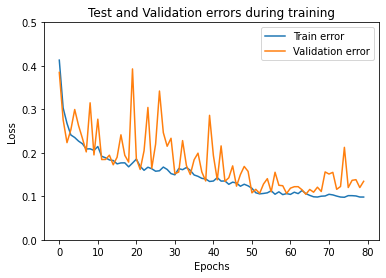
\includegraphics[width=\columnwidth]{report/images/train_validation_errors.png}
    \caption{Train and validation errors during training of the best model (6).}
    \label{fig:train_validation_errors}
\end{figure}

\begin{figure}[tbp]
    \centering
    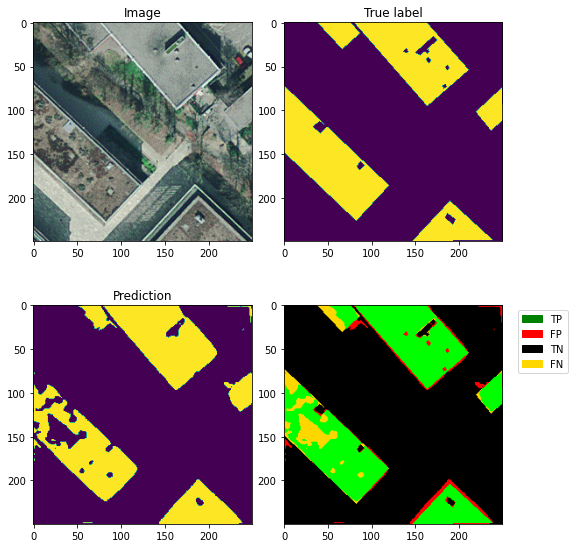
\includegraphics[width=\columnwidth]{report/images/prediction.png}
    \caption{Prediction of the best model on an image from the Test set.}
    \label{fig:prediction}
\end{figure}

\section{Discussion}
Discussion is done here.

\section{Conclusion}
Conclusion is done here.

\section*{Acknowledgements}

\bibliographystyle{ieeetr}
\bibliography{report}


\end{document}
